 \newpage
\subsection{Претензии контрагентов}
\label{BP_CLaim} 

Претензии от контрагентов поступают менеджеру по электронной почте. 

Основные проблемы связаны с качеством нанесения печати, несоблюдением геометрии изделия, наличием коробления, нарушением целостности упаковки. 

Менеджер фиксирует претензии в системе 1С: УПП, создавая документ ''Претензия покупателя'' (рис. \ref{pic:/VIIIпретензии1}), куда вносится согласно разработанной на ПРЕДПРИЯТИИ инструкции вся информацию, поступившая от клиента (рис. \ref{pic:/VIIIпретензии2}). Дополнительно формируется рассылка по электронной почте (рис. \ref{pic:/Акт 1.}).

Контрагенты должны предоставить на ПРЕДПРИЯТИЕ описание брака, фотографии бракованных изделий и маркировочные бирки (рис.\ref{pic:/Акт 2.},\ref{pic:/Акт 3.},\ref{pic:/Акт 4.}).

Отдел управления качеством на вкладке ''Рассмотрение'' в 1С: УПП (рис. \ref{pic:/VIIIпретензии3}) заносит информацию о возможных причинах выпуска брака. На вкладке ''Виновные'' указывается персонал, ответственный за выпуск претензионной продукции (рис. \ref{pic:/VIIIпретензии6}). Производится разбор причин выпуска брака с составлением акта в системе 1С: УПП (рис. \ref{pic:/VIIIпретензии5}). В акте указываются установленные причины, виновные и план корректирующих действий. Акт распечатывается и подписывается членами комиссии. Оригинал хранится в ОУК.  


%Претензии поступают менеджерам по почте или мессенджерам. 
%При поступлении официального письма от клиента менеджер делает рассылку по всем отделам, кому адресована претензия. Копия высылается в отдел ОТК и главному технологу 
%Претензии не регистрируются.
%После разбора причин выявления брака менеджер пишет ответ на официальное письмо или договаривается с заказчиком об уступках.

%В отдел ОТК претензия поступает по электронной почте от менеджера. Расследование проводят служба ОТК, находят рапорт, на эту дату и ответственного. Заметки делают прям на актеа.

%Претензии по сырью составляется службой ОТК  и передают Генеральному директору для урегулирования с поставщиками сырья.
 \newpage

 \begin{figure}
\begin{center}
 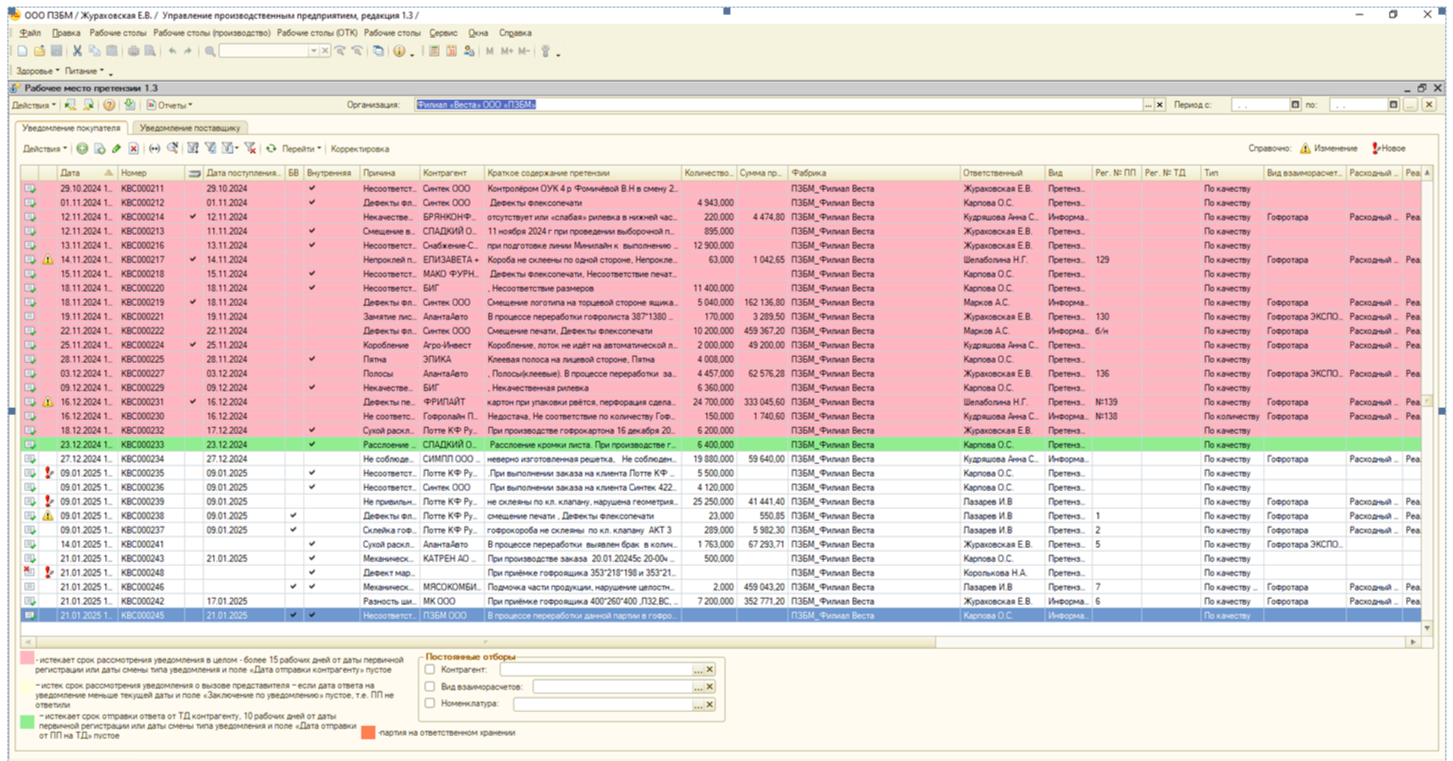
\includegraphics[height=0.35\textheight, keepaspectratio]{Pics/VIIIпретензии1.png}
\end{center}
 \caption{Журнал претензий}
 \label{pic:/VIIIпретензии1}
\end{figure}

 \begin{figure}
\begin{center}
 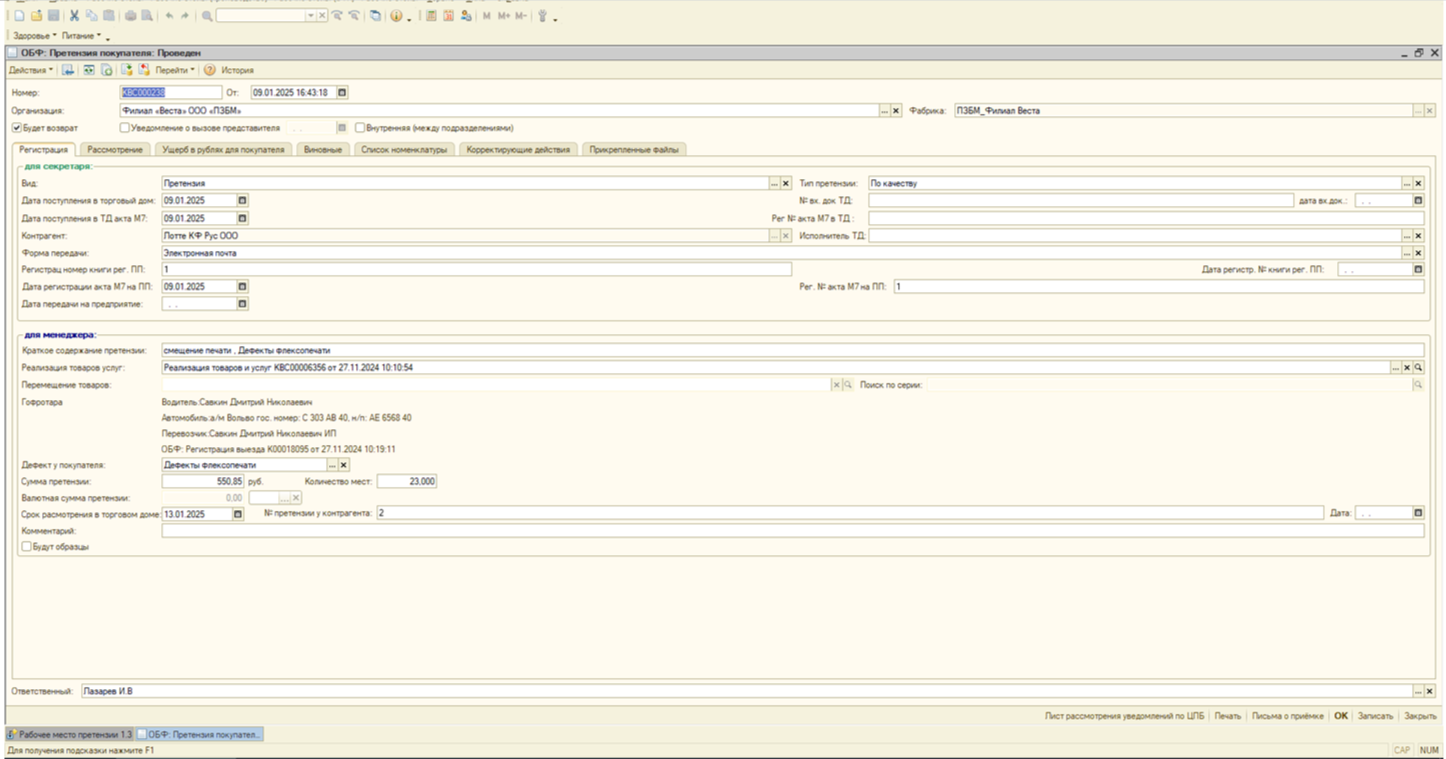
\includegraphics[height=0.35\textheight, keepaspectratio]{Pics/VIIIпретензии2.png}
\end{center}
 \caption{Вкладка ''Регистрация''}
 \label{pic:/VIIIпретензии2}
\end{figure}





\begin{figure}
\begin{center}
 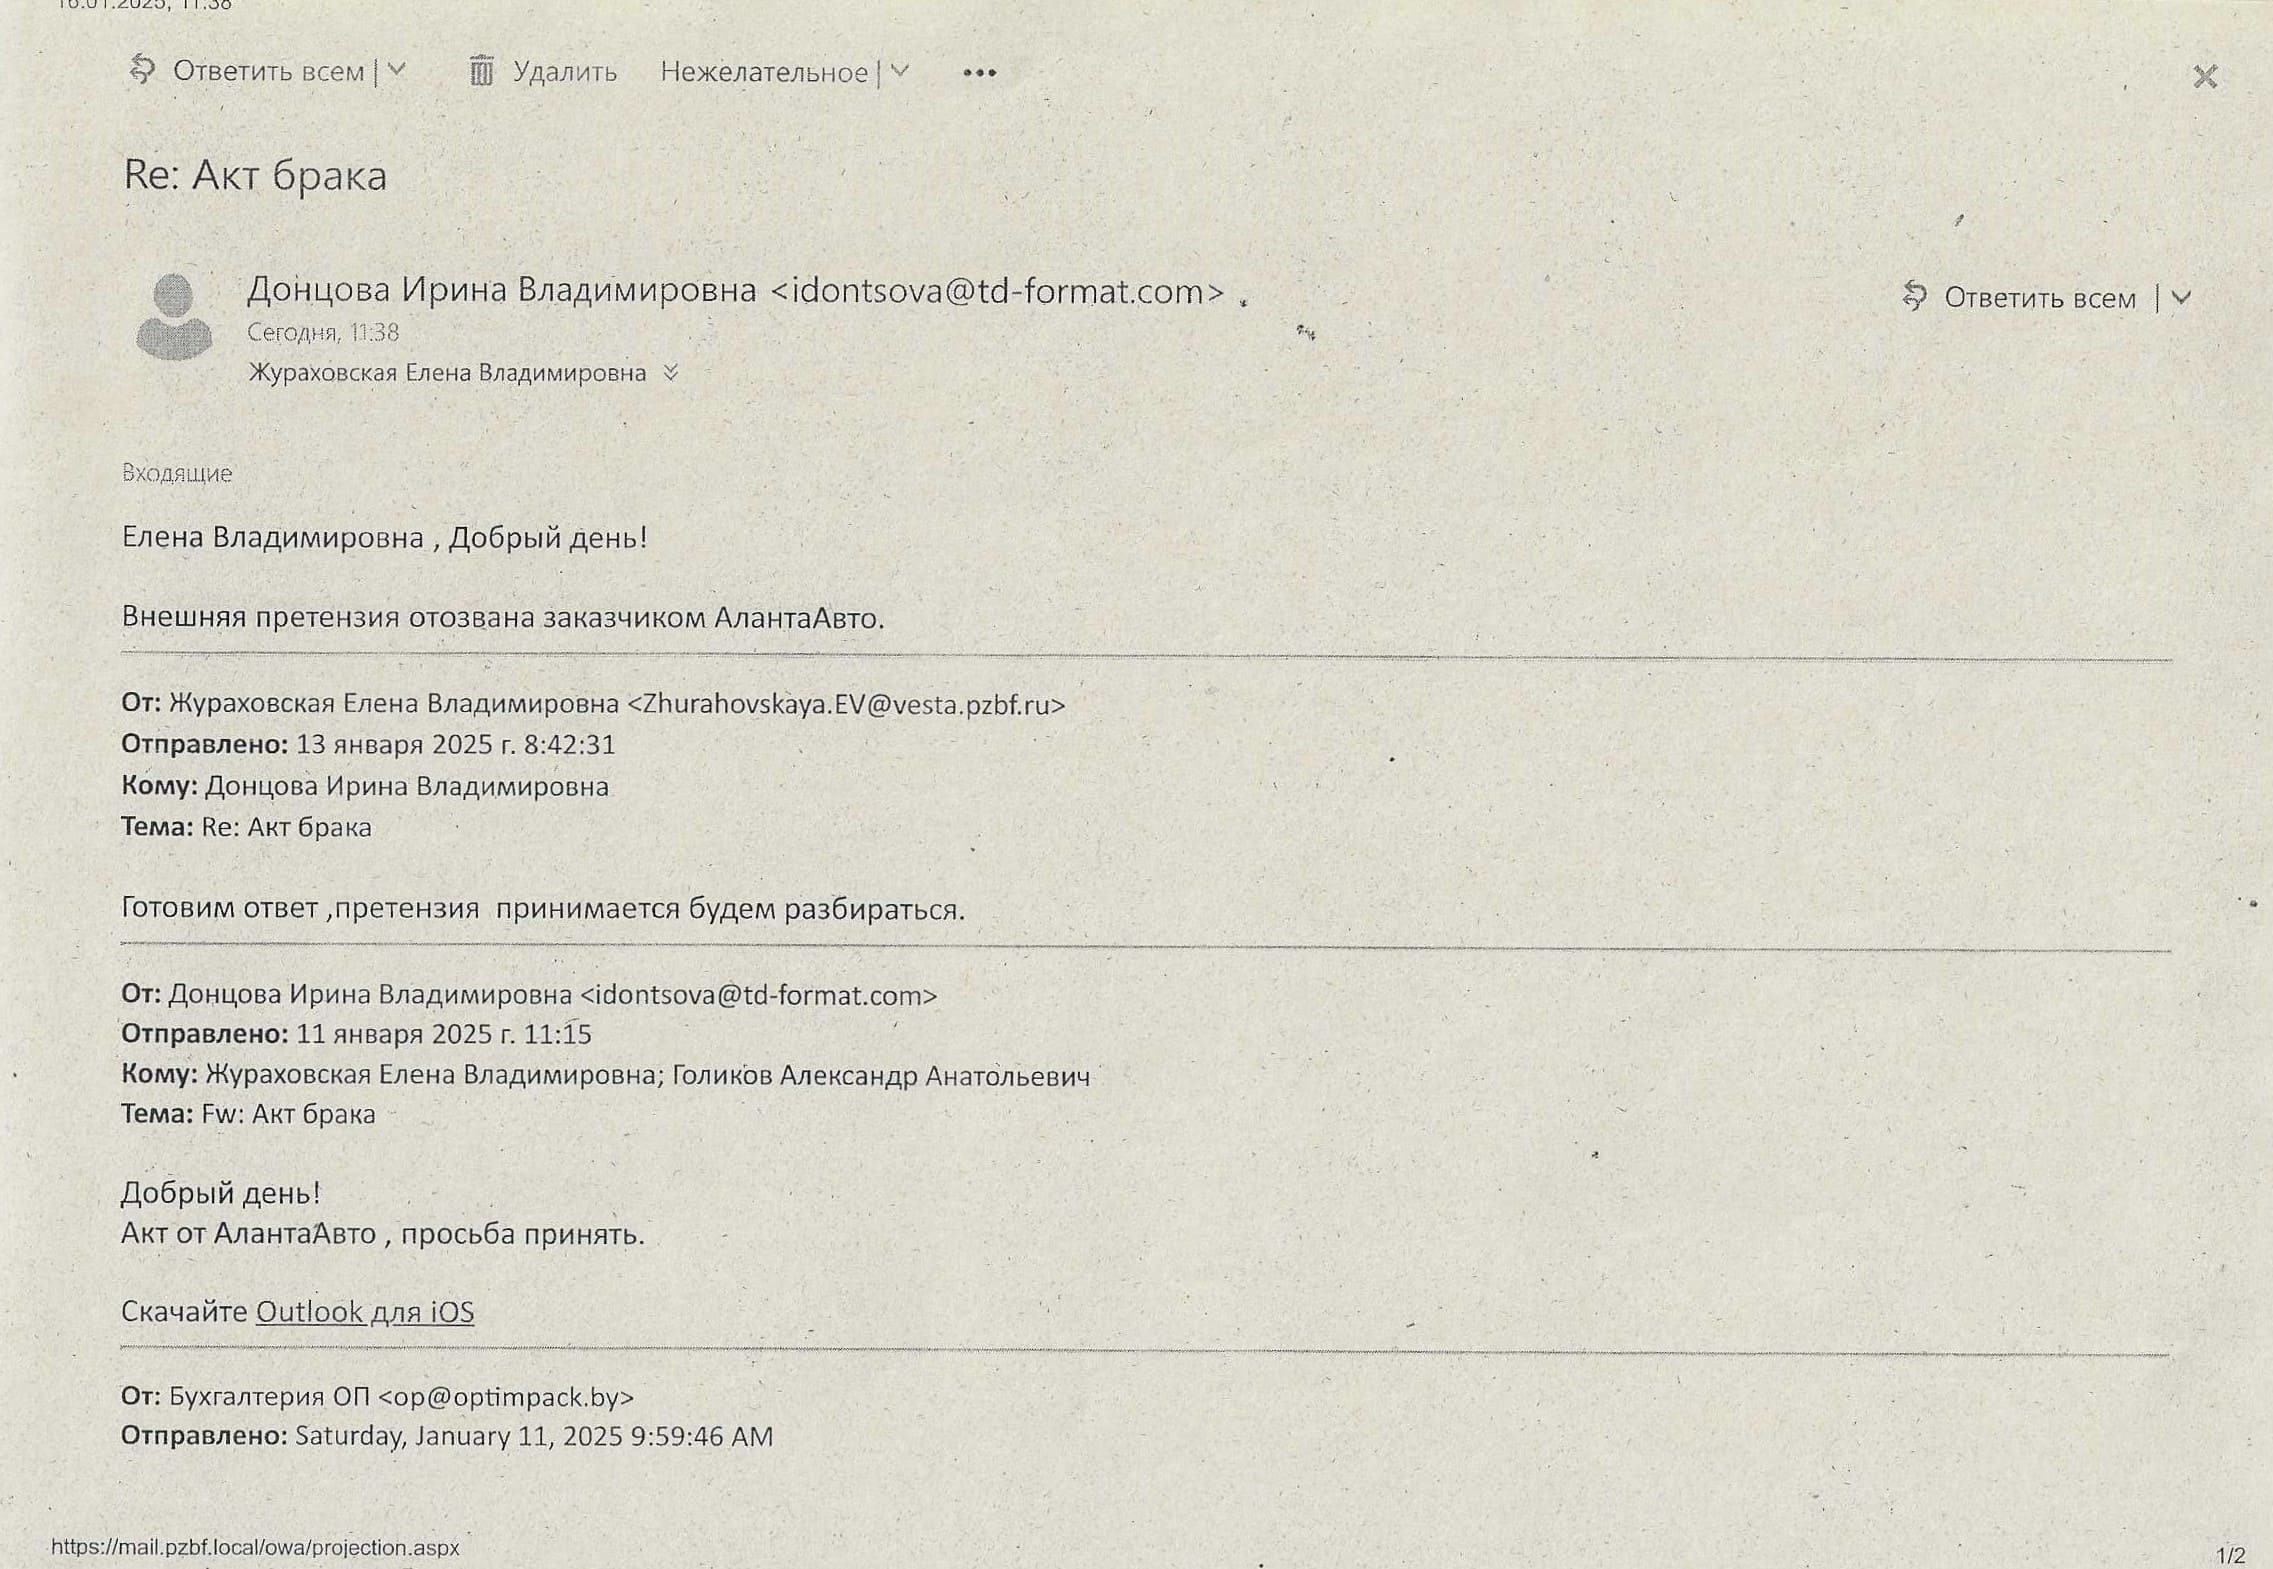
\includegraphics[height=0.45\textheight, keepaspectratio]{Pics/Акт 1.jpg}
\end{center}
 \caption{Переписка по претензии}
 \label{pic:/Акт 1.}
\end{figure}

\begin{figure}
\begin{center}
 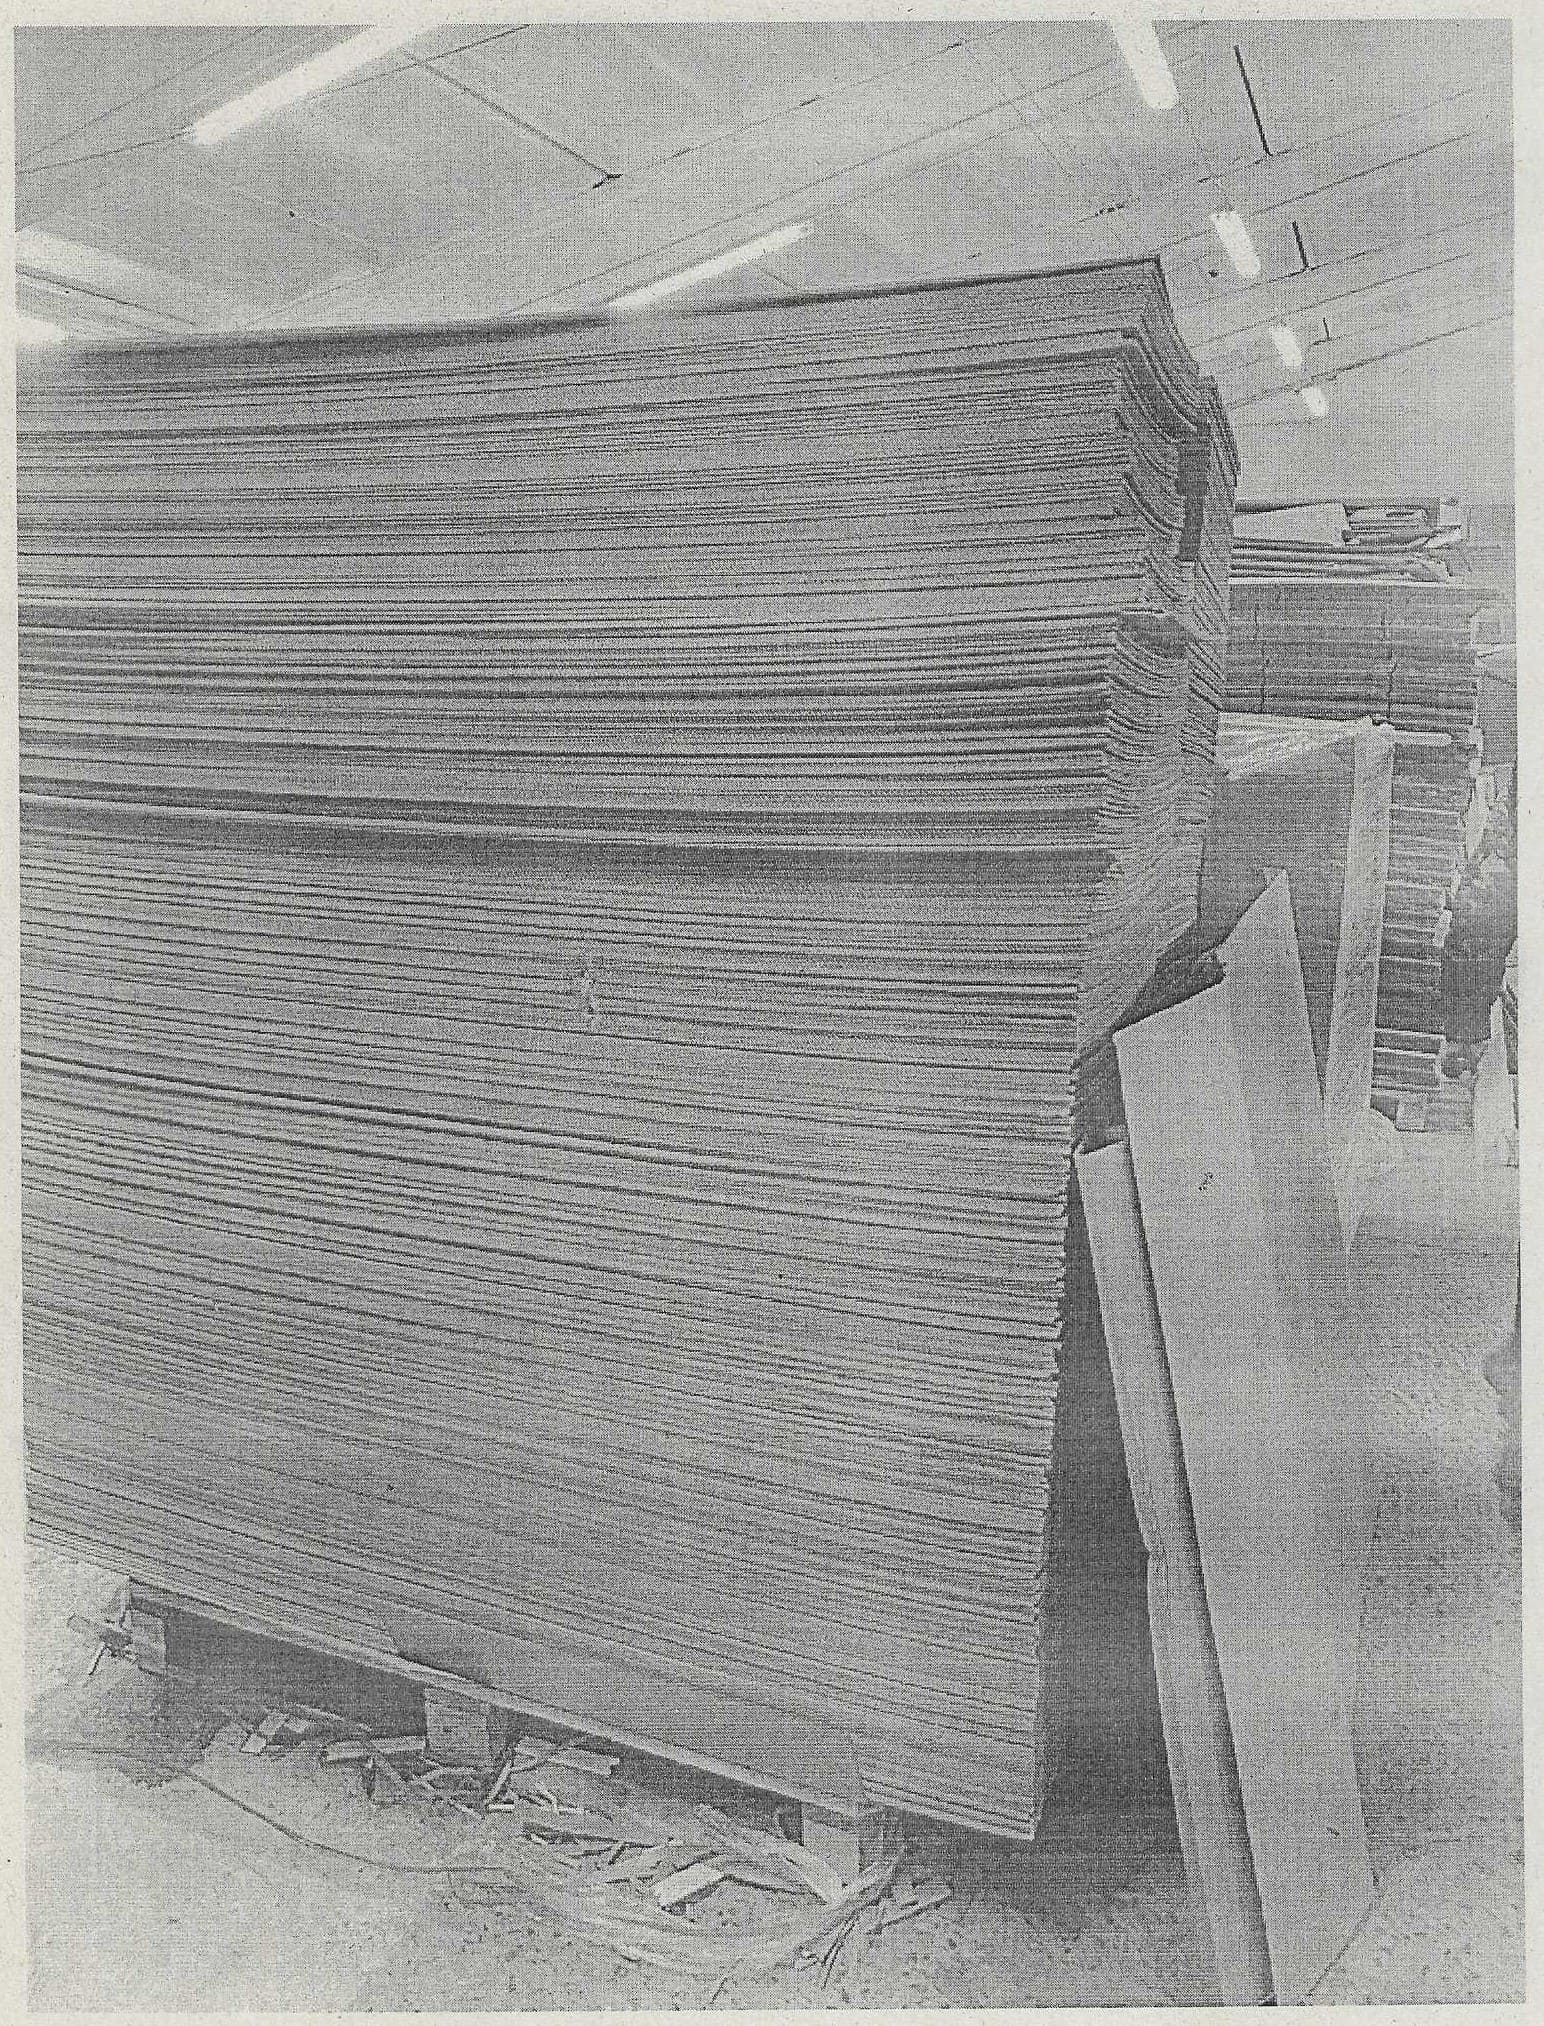
\includegraphics[height=0.9\textheight, keepaspectratio]{Pics/Акт 2.jpg}
\end{center}
 \caption{Образец претензии от клиента}
 \label{pic:/Акт 2.}
\end{figure}

\begin{figure}
\begin{center}
 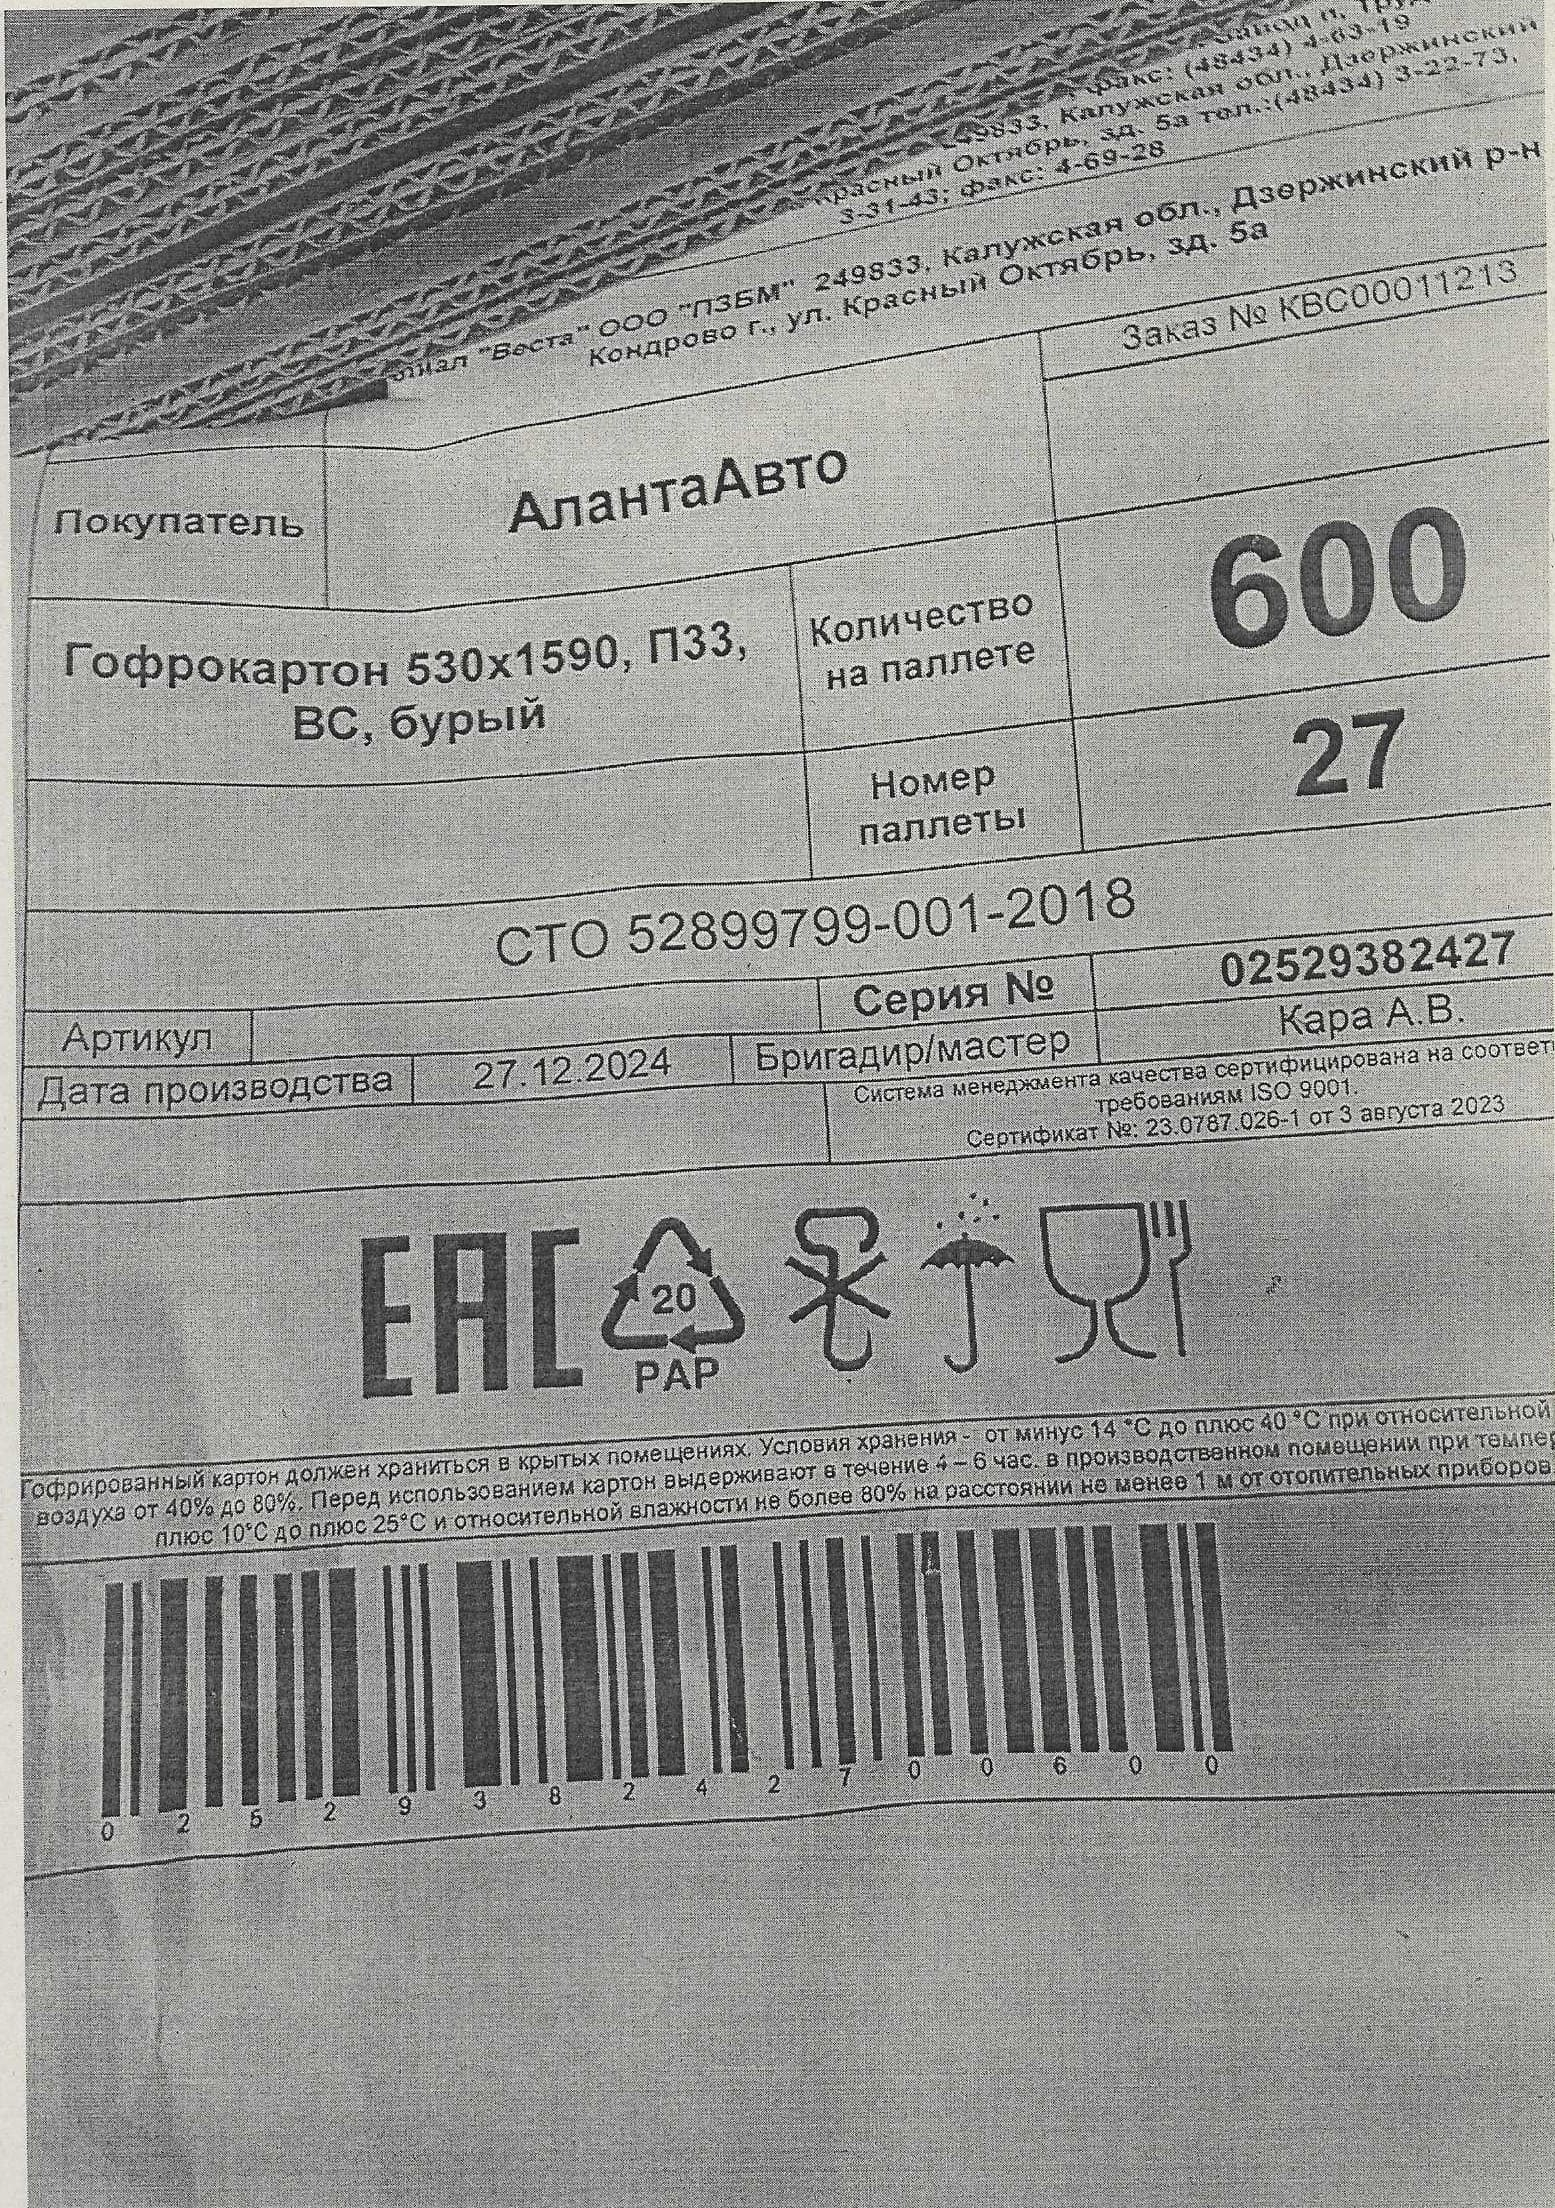
\includegraphics[height=0.9\textheight, keepaspectratio]{Pics/Акт 3.jpg}
\end{center}
 \caption{Образец претензии от клиента}
 \label{pic:/Акт 3.}
\end{figure}

\begin{figure}
\begin{center}
 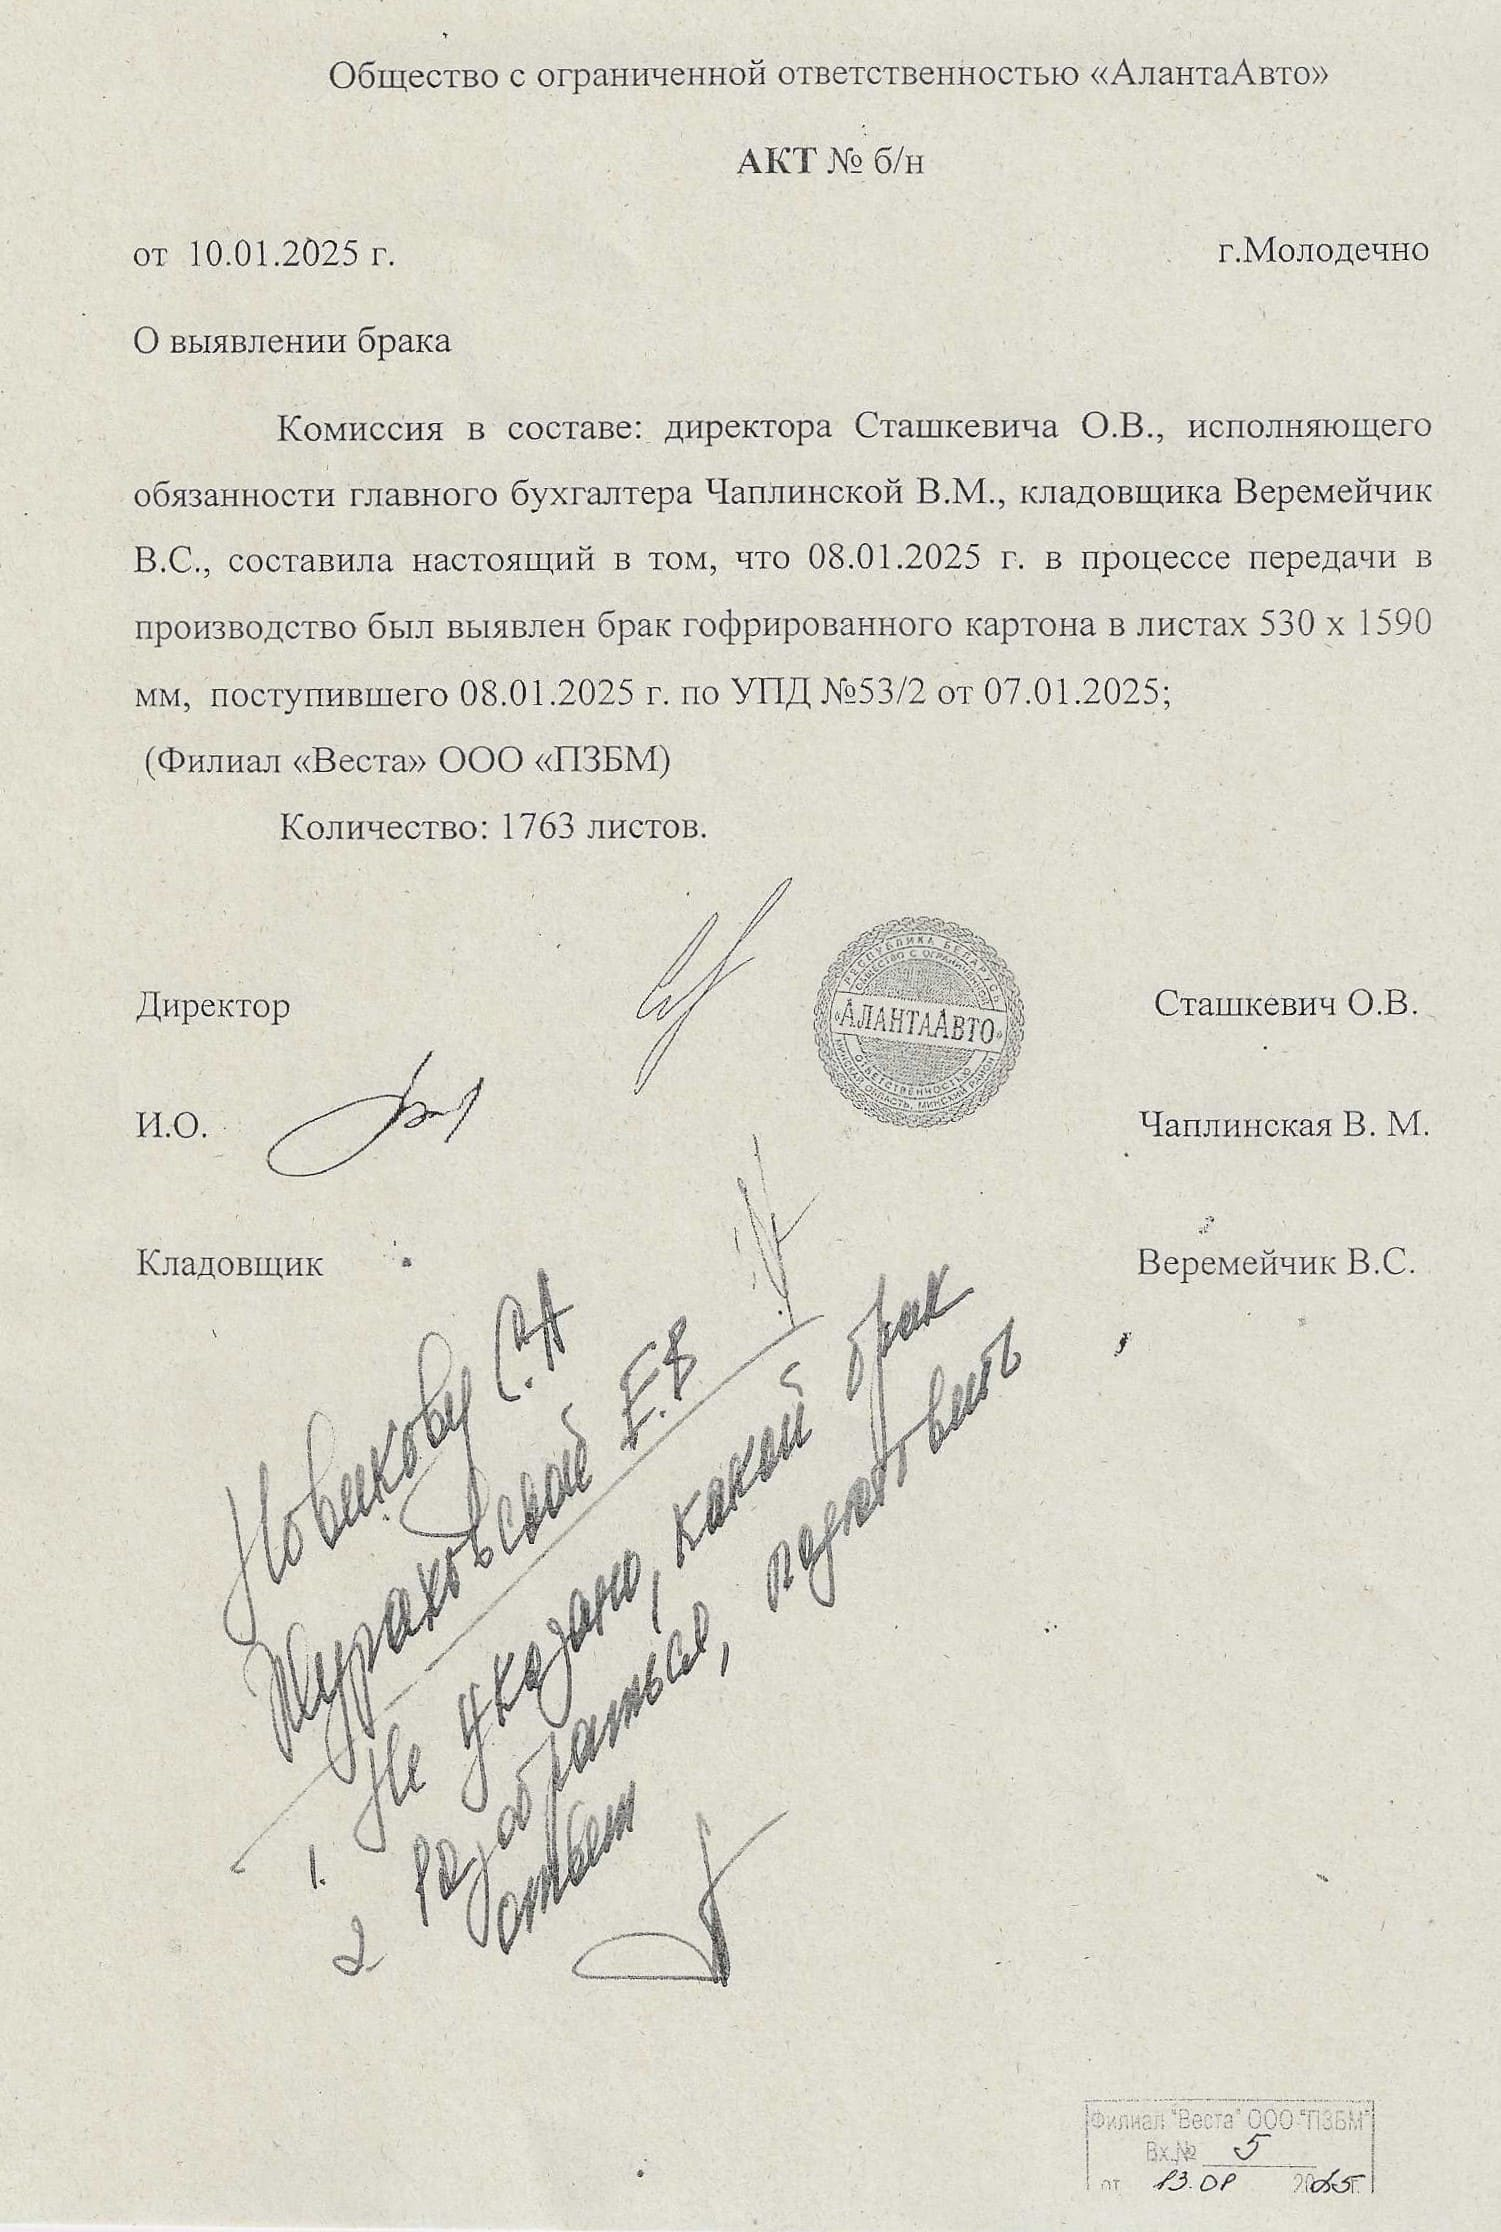
\includegraphics[height=0.9\textheight, keepaspectratio]{Pics/Акт 4.jpg}
\end{center}
 \caption{Образец претензии от клиента}
 \label{pic:/Акт 4.}
\end{figure}

\begin{figure}
\begin{center}
 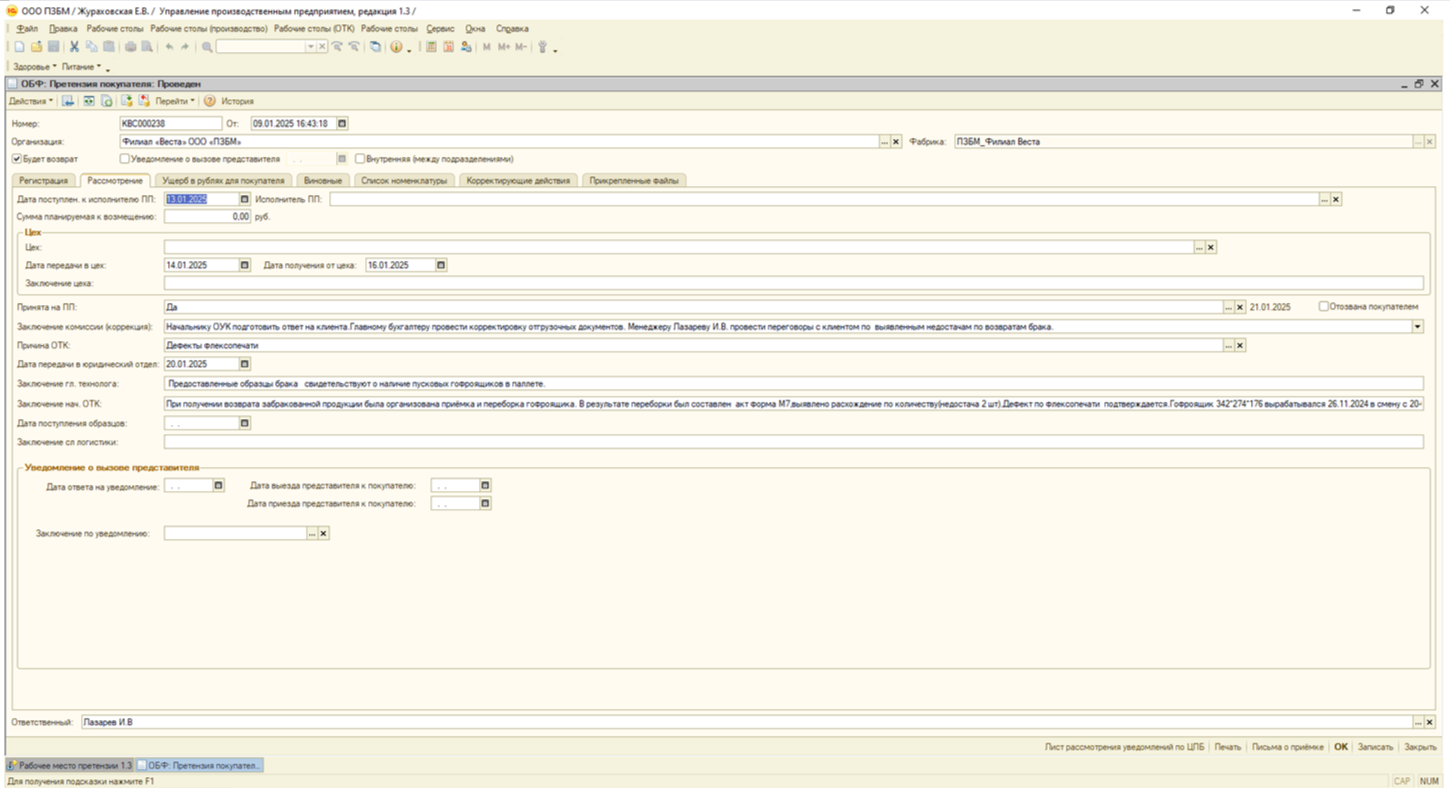
\includegraphics[height=0.35\textheight, keepaspectratio]{Pics/VIIIпретензии3.png}
\end{center}
 \caption{Вкладка ''Рассмотрение''}
 \label{pic:/VIIIпретензии3}
\end{figure}

\begin{figure}
\begin{center}
 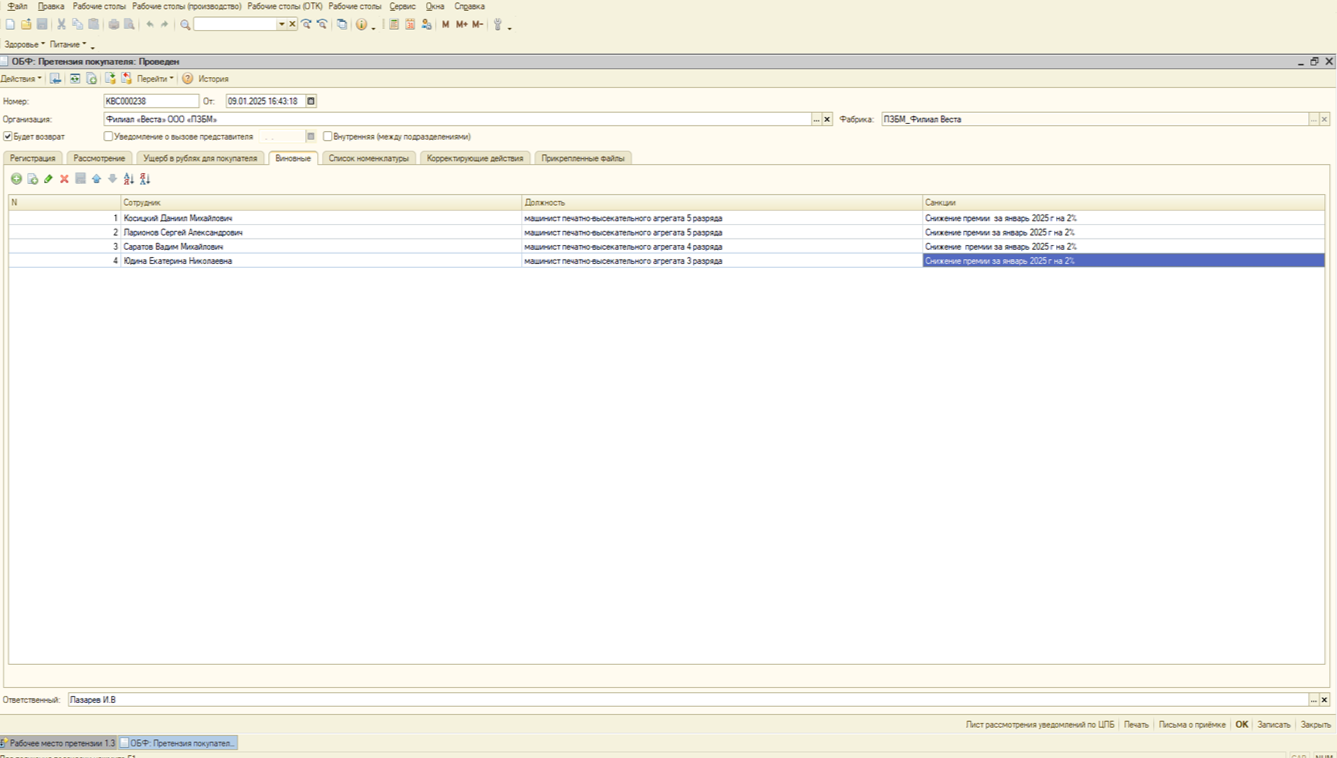
\includegraphics[height=0.35\textheight, keepaspectratio]{Pics/VIIIпретензии6.png}
\end{center}
 \caption{Вкладка ''Виновные''}
 \label{pic:/VIIIпретензии6}
\end{figure}

\begin{figure}
\begin{center}
 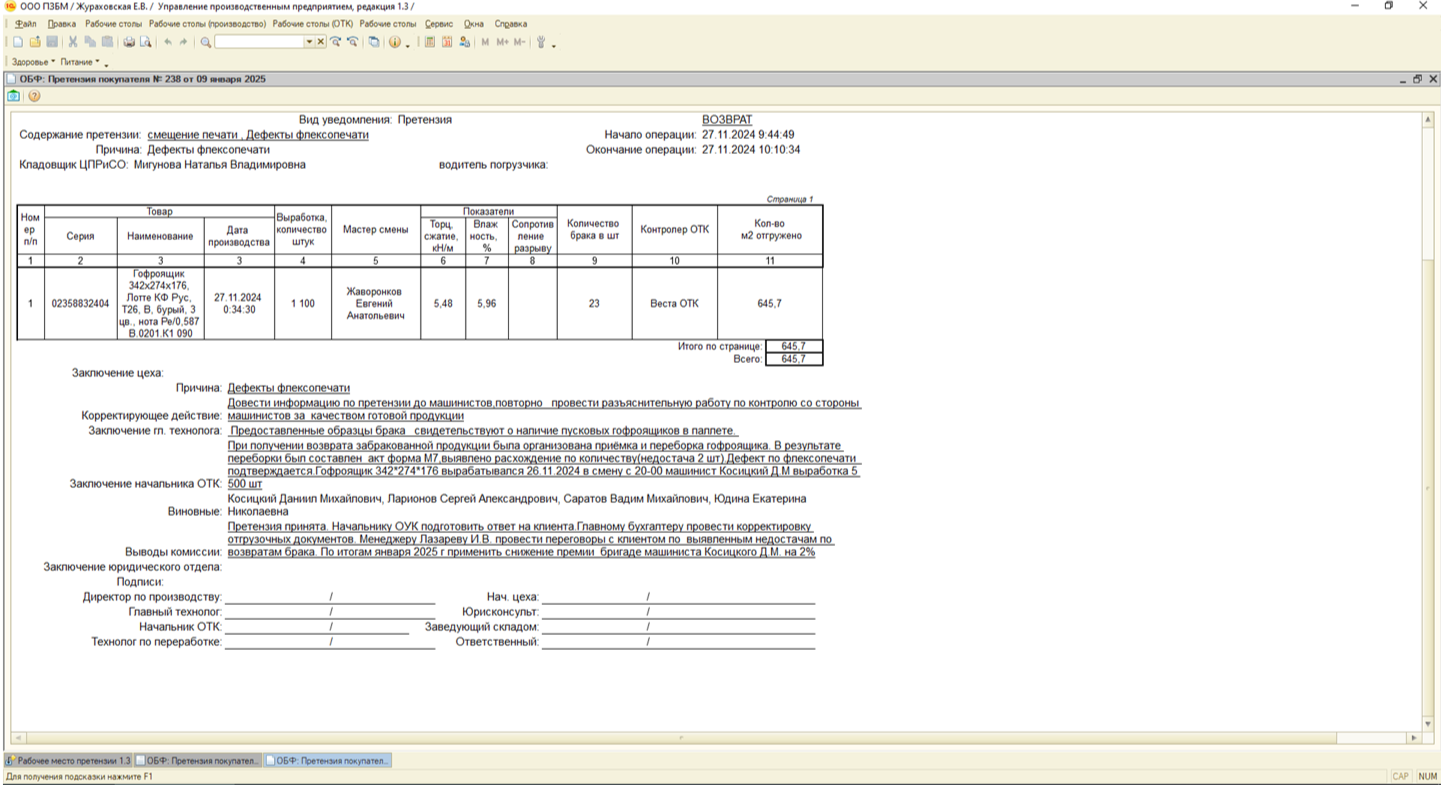
\includegraphics[height=0.35\textheight, keepaspectratio]{Pics/VIIIпретензии5.png}
\end{center}
 \caption{Акт по результатам разбора претензии}
 \label{pic:/VIIIпретензии5}
\end{figure}


\clearpage
\ifx \notincludehead\undefined
\normalsize
\end{document}
\fi